\documentclass[journal]{IEEEtran}
\usepackage[numbers]{natbib}
\usepackage{pgfplots}
\pgfplotsset{compat=1.18}
\usepackage{amsmath,amsfonts}
\usepackage{algorithmic}
\usepackage{array}
\usepackage{subcaption}
\usepackage{textcomp}
\usepackage{stfloats}
\usepackage{verbatim}
\usepackage{booktabs}
\usepackage{multirow}
\usepackage{graphicx}
\usepackage{colortbl}
% \usepackage[table,xcdraw]{xcolor}
\usepackage{tikz}
\usepackage{titlesec}
\usepackage{authblk}
\usepackage{marvosym}
\usetikzlibrary{positioning, calc}
\usetikzlibrary{arrows}
\newcolumntype{P}[1]{>{\raggedright\arraybackslash}p{#1}}

\hyphenation{op-tical net-works semi-conduc-tor IEEE-Xplore}
% \def\BibTeX{{\rm B\kern-.05em{\sc i\kern-.025em b}\kern-.08em
    % T\kern-.1667em\lower.7ex\hbox{E}\kern-.125emX}}
% \usepackage{balance}
\begin{document}
\title{bnmetamodel 2.0}

\author[1]{T. Griffiths\thanks{\textsuperscript{\Cross}Corresponding author: t.griffiths20@imperial.ac.uk}}
\author[2]{Z. Xuereb Conti}
\author[1]{M. Bluck}

\affil[1]{Department of Mechanical Engineering, Imperial College London, UK}
\affil[2]{Data-Centric Engineering / TRIC:DT, The Alan Turing Institute, UK}
\vspace{-15pt}

\maketitle

\begin{abstract}

\end{abstract}

\begin{IEEEkeywords}
Fusion power, metamodels, surrogate modelling, fusion commercialisation, machine learning, fusion economics, energy, Bayesian Networks
\end{IEEEkeywords}
\vspace{-2ex}

\section{Introduction}

Commercial-scale fusion power holds the promise of delivering reliable baseload electricity, reducing carbon emissions, and enhancing energy security. However, techno-economic modeling of future fusion power plants faces challenges due to uncertain and imprecise costing models. To address this uncertainty, probabilistic methods have been demonstrated to estimate fusion power economics effectively~\cite{Griffiths2024}.s

Despite the challenges, it's vital for the fusion community to persist in researching both technical and economic performance metrics. Fusion reactions involve intricate processes at extreme conditions within the reactor. Deterministic models must accurately capture plasma dynamics, energy transfer, and reaction kinetics, yet they often struggle to handle uncertainties inherent in fusion systems, like plasma behavior fluctuations and external factors such as magnetic field perturbations. These uncertainties can significantly impact predicted reactor performance, making consistent achievement of desired output parameters challenging. While significant advancements have been made in fusion research, our understanding of plasma physics, fusion reactions, and reactor engineering continues to evolve. Deterministic models may lack the adaptability to incorporate emerging insights or experimental data, potentially leading to discrepancies between predicted and observed reactor behavior. Failing to address these challenges could hinder investment attraction, roadmap target achievement, and the promotion of additional investment opportunities. Implementing statistical methods, like sensitivity analyses, can help assess key modeling variables, identify areas for improvement, and enhance prediction reliability.

Computational models offer a valuable tool for developing understanding in areas lacking experimental data. They provide the flexibility to simulate various scenarios and conditions rapidly, enabling quick iteration and parameter modification. This facilitates swift exploration and optimisation of designs without the need for physical modifications or repeated experiments. Given the complexity of fusion engineering systems, computational models can effectively handle numerous variables and interactions, facilitating the analysis of large-scale systems with intricate behaviours.

This study extends the computational modeling technique applied in previous research to a new case study, introducing enhancements and modifications to the methodology. The objective is to expand the application of Bayesian Networks (BNs) for a deeper understanding of fusion power design spaces. It introduces an innovative approach to managing uncertainty in fusion research, diverging from traditional techniques. The surrogate modeling aims to create a more efficient model that replicates the output of a complex model, considering its inputs and parameters. In this context, a BN acts as a surrogate for a fusion systems code, predicting the economics of fusion power plants under uncertain data, with a specific focus on Spherical Tokamaks (STs).

The use of probabilistic Bayesian inference in this analysis offers several advantages over other surrogate modeling techniques. Unlike deterministic models, Bayesian inference accounts for uncertainties in input parameters and output responses, providing a probabilistic framework that captures the inherent variability in fusion systems. Furthermore, Bayesian inference facilitates the integration of prior knowledge and observational data, enabling more robust inference and decision-making in complex engineering systems like fusion reactors. Overall, leveraging Bayesian inference allows fusion developers to extract actionable insights from limited experimental data and make informed design decisions that maximise the performance and cost-effectiveness of fusion reactor systems.

This study builds on the surrogate modeling concept introduced by Griffiths et al. (2024), shifting the focus to a new case study. It employs data from a private fusion developer to reason about uncertain economic predictions of power plants. The incorporation of multiple output nodes stands out as a key differentiator of this study, bolstering the model's ability to address multiple outputs crucial to developers. Unlike in Griffiths 2024, the input and output data from the deterministic model in this study do not emulate a future type reactor but instead one that is still in its design phase. The reason for this is to provide a more realistic and practical example of how the BN can be used to provide decision support for ongoing engineering design, enabling real-time decision-making, optimisation, and feedback for fusion developers. The study delves deeper into validation methodologies and examines the influence of hyperparameters on the results. 

The paper is structured as follows: Section~\ref{sec:background} provides a literature review of the topic, Section~\ref{sec:methodology} outlines the methodology, Section~\ref{sec:res_decision} presents the results, Section~\ref{sec:Discussion} discusses the results, and Section~\ref{sec:conc} concludes the paper. 

\section{Bayesian Networks}\label{sec:BNs}

BNs are a type of probabilistic graphical model that represents a set of variables and their conditional dependencies via a directed acyclic graph (DAG)~\cite{Hand2001}. The nodes in the graph represent the variables, and the edges represent the dependencies between the variables. The conditional dependencies are represented by the edges between the nodes. The graph structure of a BN is a compact and intuitive way to represent the joint probability distribution of the variables. The joint probability distribution is the probability of each variable in the network taking on each of its possible states. The joint probability distribution can be factorised into a product of conditional probability distributions, one for each variable given its parents in the graph. This factorisation is known as the chain rule of probability.

The chain rule of probability, also known as the general product rule, allows the calculation of any member of the joint distribution of a set of random variables using only conditional probabilities.

Given a set of random variables, say $X_1, X_2, \ldots, X_n$, the chain rule of probability states that the joint probability of these variables is the product of the conditional probabilities of each variable given all the variables that precede it. Mathematically, this can be expressed as:

\begin{align}
    P(X_1, X_2, \ldots, X_n) = & P(X_1) \nonumber \\
    & * P(X_2 | X_1) \nonumber \\
    & * P(X_3 | X_1, X_2) \nonumber \\
    & * \ldots \nonumber \\
    & * P(X_n | X_1, X_2, \ldots, X_n-1)
    \label{eq:chain_rule}
\end{align}
    
In Equation \ref{eq:chain_rule}: $P(X1, X2, \ldots, Xn)$ is the joint probability of $X1$ through $Xn$. $P(X_i | X1, \ldots, X_i-1)$ is the conditional probability of $X_i$ given all the preceding variables.

Within the problem domain, each variable is represented by a node within the DAG, where the edges of the nodes serve to represent the relationship of one node to another. Koller and Friedman explain that these DAGs can be interpreted as: \textit{a data structure, which acts as the foundational framework for efficiently representing the joint distribution in a factorised manner}. Each node in the graph represents a variable, and the directed edges indicate conditional dependencies between two variables. The parameters of a BN specify the conditional probabilities associated with each node given its parents in the network. Parameters in a BN are associated with the conditional probability distributions (CPDs) of the network's variables. A BN consists of nodes representing variables and edges representing dependencies between variables. The parameters of a BN specify the conditional probabilities associated with each node given its parents in the network. These conditional probabilities determine the relationships and dependencies between variables in the BN. By using a BN, it is not necessary to explicitly specify all the parameters of the joint probability distribution (JPD). The joint probability distribution can be factorised into a product of conditional probability distributions, one for each variable given its parents in the graph. This factorisation is known as the chain rule of probability. The structure of the BN captures the dependencies between variables, and the conditional probabilities are derived from data or expert knowledge. This allows for efficient representation of the JPD without explicitly specifying all the individual parameters, making BNs a powerful tool for probabilistic modelling. When multiple probability distributions are combined, a Joint Probability Distribution (JPD) is formed. These represent the probability of every possible combination of values of each variable. Consequently, when combined, a BN forms a structure of interdependent variables that efficiently represents a JPD without the need to explicitly specify all the parameters. This provides a compact representation by combining the \textit{local} conditional distributions for each node, with respect to its connected parent nodes~\cite{Koller2009}, see Figure~\ref{fig:BN3}.

\begin{figure}[ht]
    \centering
    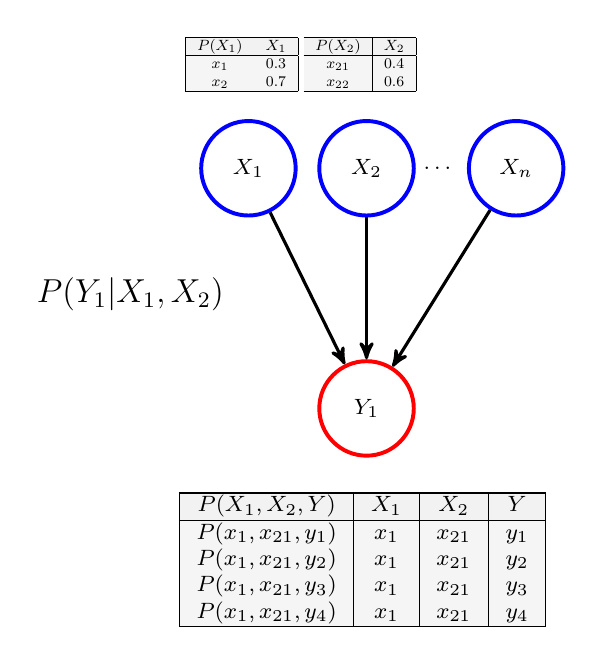
\begin{tikzpicture}[node distance=1.5cm, font=\footnotesize, align=center, >=stealth', line width=0.5mm]
        % Define colors
        \definecolor{lightgreen}{rgb}{0.56, 0.93, 0.56}
        \definecolor{lightred}{rgb}{0.98, 0.5, 0.45}

        % Nodes
        \node[draw, circle, draw=blue, text=black, minimum size=1.2cm] (input1) {$X_1$};
        \node[draw, circle, draw=blue, text=black, right of=input1, minimum size=1.2cm] (input2) {$X_2$};
        \node[right of=input2, node distance=0.9cm] (dots) {$\ldots$};
        \node[draw, circle, draw=blue, text=black, right of=dots, node distance=1cm, minimum size=1.2cm] (inputn) {$X_n$};
        % Probability expression
        \node[left of=input1, node distance=1.5cm, yshift=-1.6cm, font=\large] (prob) {$P(Y_1 | X_1, X_2)$};

        \node[draw, circle, draw=red, text=black, below=1.8cm of input2, minimum size=1.2cm] (output1) {$Y_1$};

        % Edges
        \foreach \i in {1,2,n} {
            \draw[->, line width=0.4mm] (input\i) -- (output1);  % Decreased line width
        }
        \node[above=0.2cm of input1] {
            \resizebox{1.5cm}{!}{%  <-- set the width of the table here
                \begin{tabular}{|c|c|}
                    \hline
                    \rowcolor{gray!10}
                    $P(X_1)$ & $X_1$ \\
                    \hline
                    \rowcolor{gray!8}
                    $x_1$ & 0.3 \\
                    \rowcolor{gray!8}
                    $x_2$ & 0.7 \\
                    \hline
                \end{tabular}
            }
        };

        \node[above=0.2cm of input2] {
            \resizebox{1.5cm}{!}{%  <-- set the width of the table here
                \begin{tabular}{|c|c|}
                    \hline
                    \rowcolor{gray!10}
                    $P(X_2)$ & $X_2$ \\
                    \hline
                    \rowcolor{gray!8}
                    $x_{21}$ & 0.4 \\
                    \rowcolor{gray!8}
                    $x_{22}$ & 0.6 \\
                    \hline
                \end{tabular}
            }
        };
        \node[below=0.3cm of output1] {
            %\resizebox{1.5cm}{!}{
                \begin{tabular}{|c|c|c|c|}
                    \hline
                    \rowcolor{gray!10}
                    $P(X_1, X_2, Y)$ & $X_1$ & $X_2$ & $Y$ \\
                    \hline
                    \rowcolor{gray!8}
                    $P(x_1, x_{21}, y_1)$ & $x_1$ & $x_{21}$ & $y_1$ \\
                    \rowcolor{gray!8}
                    $P(x_1, x_{21}, y_2)$ & $x_1$ & $x_{21}$ & $y_2$ \\
                    \rowcolor{gray!8}
                    $P(x_1, x_{21}, y_3)$ & $x_1$ & $x_{21}$ & $y_3$ \\
                    \rowcolor{gray!8}
                    $P(x_1, x_{21}, y_4)$ & $x_1$ & $x_{21}$ & $y_4$ \\
                    \hline
                    % Rest of the JPD table entries...
                    % ...
                \end{tabular}
            %}
        };        
       
    \end{tikzpicture}
    \caption{\small Graphical representation of BN where nodes $X_i$ represent the input variables and the node $Y_1$ represents the output variable to the analytical model. The solid lines represent the existing nodes in the model. The double-edged arrow represents additional information.}\label{fig:BN3} 
    %\vspace{-15pt}
\end{figure}

In depth, the term \textit{prior} refers to the initial probability distribution assigned to a variable. On the other hand, the \textit{posterior} probability refers to the updated probability distribution after \textit{prior} beliefs are updated via \textit{inference}, based on available evidence. The primary benefit of a probabilistic representation lies in its ability to perform \textit{probabilistic inference}, which enables bi-directional reasoning with uncertain information using probabilistic methods. Thus, adopting a BN as a surrogate model facilitates exploration of causal relationships between fusion parameters and cost in both forward and reverse directions, allowing for an uncertain fusion parameter design space to be mapped from a desired cost. 

By defining inference as the process of making deductions based on evidence, reasoning and, prior knowledge, it is possible to further characterise Bayesian inference as the act of making alterations to existing probability distributions to discover how, based on their causal relationships, the variable's remaining probability distributions are altered. This acts as a useful tool to measure and understand relationships between inputs and responses in engineering design spaces~\cite{Koller2009}. 

The interpretation of simulation outputs from analytical models can be challenging for chief (want to try and say board of directors or heads) fusion developers without a deep understanding of the associated engineering or physics principles. This can result in reliance on uncertain numerical data, without the ability to leverage the causal structure of the numerical output. In this scenario, a BN can serve as a two-way translation medium between the overall fusion research and the engineering domains. The use of bi-directional inference can assist engineers in providing feedback in the form of design parameters, based on the interconnections between the two domains. In this manner, fusion researchers can impose constraints on the output distributions of the BN, leveraging their expertise and experience, while engineers and physicists handle the input distributions to interpret engineering constraints in terms of design parameters. The `translation' process facilitated by a BN could lead to more comprehensive decisions, as probabilistic inference considers the entire network of relationships between inputs and outputs during computation. This is in contrast to traditional deterministic models, which only consider the direct relationship between inputs and outputs. 

The ability to perform bi-directional inference is a key feature of BNs, as it allows for the prediction of outputs based on input data, \textit{forward inference}, and inputs based on output data, \textit{reverse inference}. This capability is particularly useful in the context of engineering design, as it enables the exploration of causal relationships between inputs and outputs, and the prediction of inputs based on desired outputs. This can provide valuable insights for decision-making and design optimisation, as it allows for the identification of input values that are most likely to result in a desired output, and the prediction of the likely output given a set of input values.

\begin{figure*}[t]
    \centering
    \includegraphics[width=0.9\textwidth]{figures/inference_F&R_diagram.png}
    \caption{Workflow of the surrogate modelling process.}\label{fig:inference_F&R_diagram}
\end{figure*}

In addition to its flexibility and robustness, probabilistic Bayesian inference can complement current methods in fusion research by providing a holistic understanding of reactor behaviour and performance. Here are some ways this technique can be used in conjunction with current methods to enhance fusion research:

1. **Integration with Experimental Data:** Bayesian inference allows fusion researchers to seamlessly integrate experimental data, theoretical models, and expert knowledge into a unified framework. By combining various sources of information, researchers can enhance the accuracy and reliability of their predictions while quantifying uncertainties.

2. **Uncertainty Quantification:** Fusion research inherently involves uncertainties stemming from various sources such as experimental measurement errors, model approximations, and parameter variations. Bayesian inference provides a systematic approach to quantify these uncertainties, allowing researchers to assess the reliability of their predictions and identify areas where further investigation is needed.

3. **Optimisation of Experimental Design:** Bayesian methods can aid in the optimisation of experimental design by guiding researchers to select experiments that maximise information gain. Through Bayesian optimisation techniques, researchers can efficiently explore the parameter space, identify critical experiments, and prioritise resources to achieve desired research objectives.

4. **Decision Support for Design Iterations:** Fusion reactor design often requires iterative improvements to meet performance targets and address engineering challenges. Bayesian inference offers decision support tools that enable researchers to iteratively refine reactor designs based on updated information and feedback from previous iterations. This iterative process fosters continuous improvement and innovation in fusion reactor development.

5. **Risk Assessment and Management:** Fusion research involves inherent risks associated with technical uncertainties, resource constraints, and regulatory requirements. Bayesian inference facilitates risk assessment by quantifying uncertainties and evaluating the potential impact of different scenarios on reactor performance and safety. By incorporating risk analysis into the design process, researchers can proactively identify and mitigate potential risks, enhancing the overall reliability and safety of fusion reactors.

One limitation of BNs is their inability to handle continuous data. However, real-world data often comprises a mixture of discrete and continuous variables. While some implementations of BNs with continuous data have been proposed~\cite{Cobb2007,Chen2017,Li2018}, data used to configure a BN requires a discretisation process. Refer to Section~\ref{sec:design} for an overview of the discretisation method used in this study.

\subsection{Literature review}~\label{sec:background}

Include your own work from previous paper and include work from Pavonne et al 2023. 

\section{Methodology}\label{sec:methodology}

\begin{figure*}[t]
    \centering
    \includegraphics[width=\textwidth]{figures/workflow_v4.png}
    \caption{Workflow of the surrogate modelling process, adapted from~\cite{Conti2019}}~\label{fig:workflow}
\end{figure*}

In this section, steps are outlined for the creation, application of an ambiguous BN as a surrogate model. Adapated from Conti 2019 and Griffiths 2024, Figure~\ref{fig:workflow} delineates a step-wise algorithm for the creation, cross-validation, and application of BN as a surrogate model that can be applied to any input-output problem. For this study, the methodological steps are followed and explored up to step 6 in an ambiguous way i.e., no specific data is employed, it is simply to find out the best way to deploy the model, e.g., based on certain hyperparameters and validation methods. 

\subsection{\textbf{Step 1}: Define design variables}\label{sec:design}
This step involves making a strategic decision on which component or system will be the focus of the model. For instance, we might choose to model a whole reactor system, or a critical component like the breeder blanket or the divertor. The chosen component's key parameters and characteristics are then defined as input variables, denoted as $X_1$, $X_2$,\ldots, $X_n$.

Ahead of executing the selected analytical model, it requires configuration. This process includes choosing the inputs and outputs, along with defining the value ranges for each variable. The selection of inputs and outputs is guided by the objectives of the analysis and the data at hand. The value ranges for each variable are set considering the system's physical limitations and the required granularity of the analysis. Once configured, the analytical model is run to produce the dataset, which is then utilised to set up the BN. Typically, BNs perform better at making predictions when the input distribution is uniform. This is for several reasons: model assumptions: normal distributions assume a bell-shaped curve with values concentrated around a mean, while uniform distributions make no assumptions about data shape and better capture the true underlying distribution. Nonlinearity and Outliers: normal distributions are sensitive to outliers, as they can significantly impact the mean and standard deviation, which may not accurately represent the underlying relationship between variables. Uniform distributions, being less influenced by extreme values, can provide a more robust representation of the data. Flexibility and Non-parametric Modelling: Uniform distributions offer flexibility in modelling unknown or non-normally distributed data without relying on specific distribution assumptions, allowing the BN to adapt and capture complex relationships. Simplification of Model Complexity: Normal distributions require additional parameters (mean and standard deviation) that necessitate estimation, increasing model complexity and the number of parameters to learn. In contrast, using uniform distributions simplifies the model by eliminating the need for extra parameter estimation, resulting in easier training and interpretation~\cite{Duda1973,Neapolitan2004,Koller2009}.

\subsection{\textbf{Step 2}: Deterministic model}\label{sec:deterministic}
The deterministic model serves as the foundation for the BN replication. It encompasses various models, not limited to a single one, and should be capable of producing output variables denoted as $Y_1$, $Y_2$, \ldots, $Y_m$. These outputs serve as the basis for data collection and parameter estimation for the surrogate model.

\subsection{\textbf{Step 3}: Parameter Selection}\label{sec:parameters} 
This crucial step involves identifying and selecting input parameters that exert significant influence on the output variables modeled by the deterministic model. Careful consideration and expert knowledge are necessary to pinpoint the most relevant parameters that govern the system's behavior and performance.


\subsection{\textbf{Step 4}: Data Collection and Parameter Estimation}\label{sec:data} 
rministic model is executed to gather data required to configure the surrogate model. It's imperative to collect comprehensive data representing the entire design space to ensure the surrogate model's accuracy. Specific sampling techniques such as Latin Hypercube or Sobol sampling are employed to ensure the collected data adequately covers the design space. Figure~\ref{fig:sobol_vs_lhs} illustrates the sampling of the input space. The collected data is then utilized to configure the surrogate model. 

\begin{figure*}[ht]
    \centering
    \includegraphics[width=\textwidth]{figures/sobol_vs_lhs_simple.png}
    \caption{\small A comparison of the Sobol and Latin Hypercube sampling methods.}~\label{fig:sobol_vs_lhs}
\end{figure*}

\subsection{\textbf{Step 5}: Bayesian Network Configuration}\label{sec:BNconfiguration}

The BN is configured at this stage to mirror the deterministic model, using the inputs selected in step~\ref{sec:parameters} and the data collected in step~\ref{sec:data}. The data is discretised either by equidistant binning or by percentiles, for inputs and outputs respectively.

BNs are designed to handle discrete distributions, which means that datasets need to be discretised into bins before they can be used. This discretisation process is necessary to convert continuous data into discrete categories or intervals that the BN can handle effectively. This corresponds to Step 2 in Figure~\ref{fig:workflow}. By discretising the dataset into appropriate bins, the BN can leverage the discrete nature of the variables and make probabilistic inferences. Discretisation is a method used in machine learning to transform continuous variables into discrete categories or bins. For this study, two distinct methods of discretisation are employed: \textit{equal distance} and \textit{percentile binning}. For the inputs, the \textit{equal distance} approach was applied, while the \textit{percentile binning} method is implemented for the target. This differentiation allows for an effective and tailored discretisation process that accommodates the specific characteristics and requirements of the inputs and outputs.

Equal distance binning divides the range of a variable into a fixed number of equal-sized intervals or bins\@. This method assigns values to bins based on their proximity to the bin boundaries. Equal distance binning is commonly used for discretising input features in machine learning because it preserves the linear relationship between the variable values and allows for easy interpretation of the results. It can be particularly useful when the variable exhibits a linear trend or when the absolute values of the variable are important for the prediction task, making it the most appropriate method during the initial construction of the BN.\@ 

On the other hand, percentile binning divides the data based on the distribution of the variable values. Each bin contains an equal number or percentage of data points, ensuring that the bins capture an approximately equal amount of information. Percentile binning is often preferred for discretising target or output variables in ML. This is because output data distributions are typically less uniform. It can thus help handle class imbalance issues, i.e., bias, and create more balanced categories for classification tasks. By grouping data points based on their relative positions in the distribution, percentile binning can ensure that each bin represents a similar portion of the target variable, reducing the impact of outliers and enhancing model performance. Overall, the selection of the appropriate discretisation method should be based on an understanding of the data distribution, the specific machine learning task, and the goals of the analysis. 

\begin{figure}[ht]
    \centering
    \includegraphics[width=0.45\textwidth]{figures/output_dist_eg.png}
    \caption{\small An example of the output distribution of a variable demonstrating the need for percentile binning.}~\label{fig:output_dist_eg}.
\end{figure}

Once discretised into probability distributions, both inputs and outputs from training data configure the BN, corresponding to Step 3 in Figure~\ref{fig:workflow}. In this step, the BN learns the parameters and develops the causal relationships between them, i.e., populates the conditional probability tables with the prior distributions of the variables. 

In this context, the pre-configured and validated BN is employed to perform bi-directional inference. Forward inference involves updating prior assumptions of inputs, utilising available evidence to give the output response. Conversely, reverse inference involves estimating the inputs given the output. The ability to perform reverse inference stems from the fact that once a BN has learned the parameters, it no longer differentiates between inputs and outputs. This characteristic allows the network to infer in both directions, making it possible to predict inputs based on output data. This step corresponds to Step 5 in Figure~\ref{fig:workflow}.

\subsection{\textbf{Step 6}: Model Validation and Testing}\label{sec:meth_validation} 

Next, input testing data (excluding the outputs) is used to begin validation, which measures model accuracy. As part of the validation procedure and in order to avoid bias, a partitioning technique was used to partition the dataset into training and testing in $k$ distinct manners, known as $k$-fold cross-validation. This means the BN was built, and then validated $k$ times, with $k$ unique combinations of training and $k$ testing sets. The ratio of the split between training and testing sets in each fold is determined by the number of folds used to split the dataset by $1/k$, e.g., 3 folds will have a test split size of $1/3 = 33\%$. The validation itself corresponds to Step 4 in Figure~\ref{fig:workflow}, however the dataset is split after discretisation (Step 2), and ahead of BN configuration (Step 3). 

In order to quantify how well the model makes predictions compared to the analytical response, the predicted values were compared with the actual values in the testing data. In traditional machine learning evaluation methods like Root Mean Square Error (RMSE), the predictions and actual values are typically scalar values, such as numerical measurements or continuous variables. However, in the context of BNs, the outputs are probabilistic, distributions, or categorical variables rather than single numerical values. As a result, standard evaluation metrics like RMSE are not directly applicable, and alternative or custom approaches must be used to assess the performance of BN models. This can done either by (i) calculating the difference between the mean of the predicted bin and the simulated value in the testing data, $d_{1}$, (ii) calculating the difference between the mean of the predicted bin and the mean of the bin in which the actual simulated value lies, $d_{2}$. See [FIG].

The NDE is a measure used to assess the relative magnitude of the distance error in relation to the range of values in a given bin. It helps to put the distance error into perspective and make it comparable across different bin ranges. By dividing the distance error by the difference between the maximum and minimum bin range values, a normalised distance error is obtained that takes into account the scale and range of the data. This normalisation allows for a fair comparison of the distance error across different bin ranges, providing a standardised measure of the error~\cite{Conti2019}.

\subsection{\textbf{Step 7}: Design Constraint Decision Support}\label{sec:meth_decision}

Here the application of the BN to provide decision support for engineering design is discussed, such as determining input ranges for optimal performance based on a desired output using reverse inference. This demonstrates an update from previous work with greater depth and analysis given. 

\section{Validation of the Bayesian Network}\label{sec:res_validation}
Here, the results of applying the methology from Section~\ref{sec:methodology} are presented. Section~\ref{sec:res_validation} provides an overview of the outcomes obtained through $k$-fold cross-validation. Section~\ref{sec:res_hyperparameter} presents the findings from hyperparameter tuning. 

To enable $k$-fold cross-validation, the dataset was split into 10 folds. 10 fold cross-validation aligns with the recommendation by Marcot et al.~\cite{Marcot2021}, who support the prevalent use of $k$=10 for BNs in literature. Plotting the NDE in a histogram provides a good illustration of model performance, see Figure~\ref{fig:k-foldhistograms}. The resulting validation plot distributions in~\ref{fig:k-foldhistograms} provide an intuitive indication of how well the BN predicts the numerical responses. Overall, when observing the distribution of the d1 plots for all 10 folds, it can be noted that the BNM built on 10,000 data points, seems to predict the correct response with an average 84\% accuracy.

The implementation of $k$-fold cross-validation, specifically with $k$=10 as recommended by Marcot et al.\cite{Marcot2021}, has proven to be effective in assessing the performance of the Bayesian Network Meta-model (BNM). The Normalised Distance Error (NDE), visualised through a histogram (Figure\ref{fig:k-foldhistograms}), offers a clear representation of the model's predictive capabilities.

The validation plot distributions in Figure~\ref{fig:k-foldhistograms} provide an intuitive understanding of the model's proficiency in predicting numerical responses. A closer examination of the d1 plots across all 10 folds reveals a noteworthy observation: the BNM, when constructed with 10,000 data points, demonstrates a high predictive accuracy, averaging at 95\%.

This high level of accuracy underscores the model's robustness and reliability in making predictions. It also highlights the value of using a substantial dataset for building the model. These findings contribute to the growing body of evidence supporting the use of BNss in making accurate predictions, and they underscore the importance of careful model construction and validation.

\begin{figure*}
    \centering
    \includegraphics[width=\textwidth]{figures/TE_results/D1kfold.png}
    \caption{\small Normalised probability histograms with prediction accuracy values for each fold is shown for $d_{1}$ bin resolution = 7, dataset size = 10240.}~\label{fig:k-foldhistograms}
\end{figure*}

\subsection{Hyperparameter Tuning}\label{sec:res_hyperparameter}
Using the data, calibration of hyper-parameters (such as bin resolution and dataset sizes) were examined by exploring two factors: (i) utilising three distinct dataset sizes and, (ii) experimenting with different bin resolutions during discretisation. The objective was to determine how modifying these paramters impacted the BN's ability to make predictions that could be usefully interpretted by the user. Consequently, for (i) this meant dataset sizes of 1400, 5120, and 10240 and, for (ii), incrementally increasing the number of bins used in discretisation between inputs and outputs for all combinations between 3 and 12, respectively. For (i), it was found that configuring the BN using the largest dataset resulted in the highest prediction accuracy. For (ii) the findings are presented in~\ref{fig:3D_SA_trimmed_39_D1}, illustrating that the model exhibited optimal performance when and input data was discretised into 7 bins and output data into 5 bins, respectively. In general, the average prediction accuracy for $d_{2}$ errors tends to be higher than that for $d_{1}$ errors, except in the case of using high bin resolutions.

\begin{figure}[h]
    \centering
    \includegraphics[width=\columnwidth]{figures/SA_3D_trimmed_39.png}
    \caption{\small A 3D surface plot displaying the average accuracy of predictions for $d_{1}$ errors while investigating variations in bin resolution.}~\label{fig:3D_SA_trimmed_39_D1}
\end{figure}

Using the data, calibration of hyper-parameters (such as bin resolution and dataset sizes) were examined by exploring two factors: (i) utilising three distinct dataset sizes and, (ii) experimenting with different bin resolutions during discretisation. The objective was to determine how modifying these paramters impacted the BN's ability to make predictions that could be usefully interpretted by the user. Consequently, for (i) this meant dataset sizes of 1400, 5120, and 10240 and, for (ii), incrementally increasing the number of bins used in discretisation between inputs and outputs for all combinations between 3 and 12, respectively. For (i), it was found that configuring the BN using the largest dataset resulted in the highest prediction accuracy. For (ii) the findings are presented in~\ref{fig:3D_SA_trimmed_39_D1}, illustrating that the model exhibited optimal performance when and input data was discretised into 7 bins and output data into 5 bins, respectively. In general, the average prediction accuracy for $d_{2}$ errors tends to be higher than that for $d_{1}$ errors, except in the case of using high bin resolutions.

The results from the hyper-parameter calibration provide valuable insights into the performance of the BN model. Two key factors were examined: dataset size and bin resolution during discretisation. The investigation found that the size of the dataset used to configure the BN significantly impacts its predictive accuracy. Specifically, the largest dataset (10,240) yielded the highest prediction accuracy. This suggests that the BN model benefits from a larger volume of data, likely because it provides a more comprehensive representation of the underlying distributions and dependencies. Whilst this is not a groundbreaking realisation, it is a useful reminder that the quality of the data used to configure the BN is crucial to its performance. The findings also highlight the importance of collecting a sufficient amount of data to ensure the model's accuracy and reliability, and ensures that these models are not overfitting to the training data. Going forward, this study will inform the collection of data for future BN models, ensuring that the dataset is sufficiently large to support accurate and reliable predictions, especially when the model is used to make critical decisions in engineering design with fusion developers.

The bin resolution during discretisation also played a crucial role in the model's performance. The optimal performance was observed when the input data was discretised into 7 bins and the output data into 5 bins. This indicates a balance is needed in the bin resolution. Too few bins may oversimplify the data, losing important information, while too many bins can lead to overfitting, where the model becomes too tailored to the training data and performs poorly on new data.

Interestingly, the average prediction accuracy for $d_{2}$ errors was generally higher than that for $d_{1}$ errors, except when using high bin resolutions. This is largely down to how the model handles the different types of errors. The $d_{1}$ error measures the difference between the mean of the predicted bin and the simulated value in the testing data, while the $d_{2}$ error measures the difference between the mean of the predicted bin and the mean of the bin in which the actual simulated value lies. Thus, the likelihood that the correct bin is predicted is higher for $d_{2}$ errors, as it is based on the mean of the bin rather than the actual value. This is an important consideration when interpreting the results and understanding the model's performance. The results suggest that the model may be more sensitive to the bin resolution for $d_{1}$ errors, and care should be taken when choosing the bin resolution in this case.

These findings contribute to a deeper understanding of how hyper-parameter choices affect the performance of BN models, and can guide the selection of these parameters in future work by providing a clear indication of the optimal dataset size and bin resolution to benchmark the model. This will help to ensure that the BN model is configured to provide accurate and reliable predictions, and that the results can be interpreted with confidence.

\section{Case Study Appplication: Component Decision Support}\label{sec:res_decision} 

\begin{figure*}[t]
    \centering
    \includegraphics[width=0.8\textwidth]{figures/4grid_scatter.png}
    \caption{\small A 4x4 scatter-grid to illustrate the sampling of an example input space. The scatter-grid is a visual representation where each point represents a unique combination of input values. The scatter-grid is a useful tool for visualising the distribution of the input space and identifying any gaps or biases in the data.}\label{fig:scatter_sampling}
\end{figure*}

Section~\ref{sec:res_reverse} delves into the outcomes of reverse inference with the BN, emphasising the prediction of ranges for economic fusion parameters while considering uncertainties in capital cost. Results from the model provide decision support for components, such as determining input ranges for optimal performance based on a desired output using reverse inference. Lastly, Section~\ref{sec:res_decision} presents the application of the results from reverse inference to provide decision support for engineering design, such as determining input ranges for optimal performance based on a specified output. This demonstrates an update from previous work with greater depth and analysis given in Step 7 (~\ref{sec:meth_decision}).

For Step 1: Define Design Variables (\ref{sec:design}), the system modelled was a whole reactor. The purpose was to determine how important output parameters vary with certain inputs by studying their sensitivity to one another. For Step 2, (~\ref{sec:deterministic}), the deterministic  model used was `PyTOK', a systems code that finds optimum working point using a series of 0D and 1D approximations that model all subsystems. Previous studies from Griffiths et al. 2024 have shown that PROCESS is a suitable model for this step, and any input-output model could be used in it's place. For Step 3 (\ref{sec:parameters}), the important parameters for the surrogate model were carefully selected based on insights from the PyTOK model, a comprehensive tool for fusion reactor analysis. The chosen input parameters include:

\begin{itemize}
    \item \textbf{Major Radius ($R$)}: This parameter represents the distance from the center of the torus to the center of the plasma. In fusion terminology, it defines the size of the plasma confinement region and influences key plasma stability characteristics. A larger major radius typically allows for increased plasma volume, enhancing overall fusion performance. 
    \item \textbf{Aspect Ratio ($A$)}: The aspect ratio signifies the ratio of the major radius ($R$) to the minor radius ($a$), which is the radius of the cross-sectional circle of the torus. Higher aspect ratios are characteristic of spherical tokamaks, a specific type of fusion device. Aspect ratio plays a crucial role in shaping the plasma equilibrium and can affect plasma stability and confinement properties. 
    \item \textbf{Effective Ion Charge ($Z_{\text{eff}}$)}: This parameter serves as a measure of the average charge state of ions within the plasma. It is calculated by summing the square of the charge of each ion species, weighted by their respective densities. A higher effective ion charge may indicate the presence of impurities in the plasma, which can lead to increased energy losses and impact fusion performance. 
    \item \textbf{Toroidal Field on Plasma ($B_{\text{T}}$)}: The toroidal field refers to the magnetic field that wraps around the torus in the direction of the major radius ($R$). It plays a crucial role in confining the plasma along the toroidal direction and is typically much stronger than the poloidal field, which confines the plasma in the radial direction. The strength of the toroidal field influences plasma stability, confinement, and overall fusion performance.
\end{itemize}

The chosen output parameters were:

\begin{itemize}
    \item \textbf{Engineering Gain ($Q_{\text{eng}}$)}: This factor is defined as the ratio of the power produced by the fusion reactions to the external heating power.  Thus, a $Q_{\text{eng}}$=1 represents breakeven, where the power generated from fusion reactions in a plasma exceeds that of the external power needed to create the plasma state. Achieving a high $Q_{\text{eng}}$ is indicative of the reactor's ability to sustain fusion reactions efficiently. 
    \item \textbf{High Grade Waste Heat ($H$) (MWt)}: This represents the amount of usable heat energy produced at a high temperature by the fusion reaction. It can be harnessed for various applications such as industrial processes, district heating, or additional power generation. Efficient utilisation of waste heat maximizes the overall energy output and efficiency of the fusion reactor.
    \item \textbf{Net Electrical Output ($E$) (MWe)}: This parameter quantifies the amount of electrical power generated by the fusion reactor. Achieving a high $E$ signifies the effectiveness of the fusion reaction in producing usable electrical energy.
    \item \textbf{Capital Cost ($C$) (million USD)}: This represents the overnight cost of building the fusion reactor. It is a crucial factor in assessing the economic feasibility and viability of implementing fusion energy technology.
\end{itemize}

Achieving a high $E$ signifies the efficiency and effectiveness of the fusion reaction in generating usable electrical energy. --A reactor with an elevated $E$ can contribute significantly to the power grid, meeting energy demands and reducing reliance on fossil fuels or other non-renewable sources-- reword this for different context. $H$ refers to the thermal energy produced by the fusion reaction at a temperature suitable for efficient conversion into usable heat or electricity. This waste heat can be utilised for various industrial processes, district heating, or power generation, maximising the reactor's energy output and overall efficiency [citation of my own work]. $Q_{\text{eng}}$ represents the ratio of the power output from the fusion reaction to the power input required to sustain the reaction. A high $Q_{\text{eng}}$ indicates that the fusion reactor is producing significantly more energy than it consumes, making it a viable and sustainable energy source.

For Step 3 (\ref{sec:data}), The input space was sampled between the parameter limits using Saltelli's extension of the Sobol sequence [CIATIONS], a quasi-random low-discrepancy sequence used to generate pseudo-uniform samples of parameter space. Data was collected from the PyTOK model to produce a dataset size of 10,000. See Figure~\ref{fig:scatter_sampling}.

For~\ref{sec:BNconfiguration}, the BN was configured to replicate the deterministic model using the inputs outlined in above for~\ref{sec:parameters}, see Figure~\ref{fig:BN2}.

\begin{figure}[h]
    \centering
    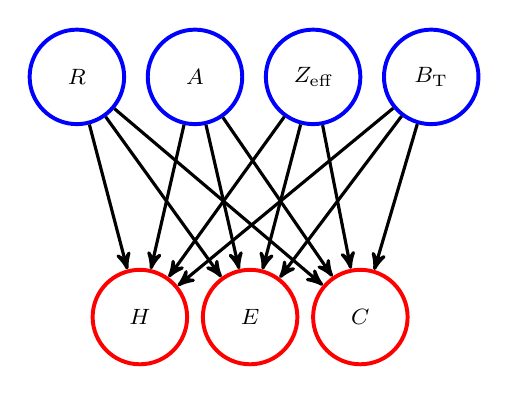
\begin{tikzpicture}[node distance=1.5cm, font=\footnotesize, align=center, >=stealth', line width=0.5mm]
        % Define colors
        \definecolor{lightgreen}{rgb}{0.56, 0.93, 0.56}
        \definecolor{lightred}{rgb}{0.98, 0.5, 0.45}

        % Nodes
        \node[draw, circle, draw=blue, text=black, minimum size=1.2cm] (input1) {$R$};
        \node[draw, circle, draw=blue, text=black, right of=input1, minimum size=1.2cm] (input2) {$A$};
        \node[draw, circle, draw=blue, text=black, right of=input2, minimum size=1.2cm] (input3) {$Z_{\text{eff}}$};
        \node[draw, circle, draw=blue, text=black, right of=input3, minimum size=1.2cm] (input4) {$B_{\text{T}}$};

        \node[draw, circle, draw=red, text=black, below=1.8cm of input2, xshift=-0.7cm, minimum size=1.2cm] (output2) {$H$};
        \node[draw, circle, draw=red, text=black, below=1.8cm of input2, xshift=0.7cm, minimum size=1.2cm] (output3) {$E$};
        \node[draw, circle, draw=red, text=black, below=1.8cm of input2, xshift=2.1cm, minimum size=1.2cm] (output4) {$C$};

        % Edges
        \foreach \i in {1,...,4} {
            \foreach \j in {2,...,4} {
                \draw[->, line width=0.4mm] (input\i) -- (output\j);  % Decreased line width
            }
        }
    \end{tikzpicture}
    \caption{\small Graphical representation of Bayesian Network where nodes represent the input variables (Major Radius $R$, Aspect Ratio $A$, Effective Ion Charge $Z_{\text{eff}}$, Toroidal Field on Plasma $B_{\text{T}}$) and the output variables (High Grade Wasteheat $H$, Net Electrical Output $E$, Capital Cost $C$) to the analytical model.}\label{fig:BN2} 
    \vspace{-15pt}
\end{figure}

%%\subsection{Forward Inference}\label{sec:res_forward}
\subsection{Bayesian Reverse Inference}\label{sec:res_reverse}

This section presents the outcomes of reverse inference, a method employed to predict the input parameters that are most likely to yield a specified output, such as minimising $C$. In this context, modelling a reactor with elevated $E$, $H$, and $Q_{\text{eng}}$ within specific ranges is indicative of aiming for a high-performance reactor system. 

Analysis of a reactor system with such output parameters presents several challenges, particularly in deterministic models. Deterministic models face challenges in accurately capturing the complex dynamics of fusion reactions, including plasma confinement, energy transfer mechanisms, and reaction kinetics. These models often struggle to account for inherent uncertainties and variabilities in fusion systems, such as fluctuations in plasma behavior and external factors like magnetic field perturbations. As our understanding of plasma physics and reactor engineering continues to evolve, deterministic models may lack the flexibility to adapt to emerging insights or experimental data, potentially leading to discrepancies between predicted and observed reactor behavior.

In contrast, probabilistic Bayesian inference offers a more flexible and robust approach to modeling fusion reactors. By incorporating uncertainties and prior knowledge into the analysis, Bayesian inference allows for probabilistic assessments of reactor performance and facilitates the exploration of the design space under varying conditions. This probabilistic framework enables researchers to account for uncertainties, optimise reactor designs, and make informed decisions to achieve desired output parameters while mitigating risks associated with deterministic modeling limitations.

$C$, was increased between each result, ranging from \$3.4-3.8 billion to \$4.4-6.5 billion. The aim of this approach was to illustrate the variation in the posterior distributions of the input parameters contingent on $C$. The outcomes of the reverse inference are depicted in Figures~\ref{fig:BN_case_study} and~\ref{fig:BN_case_study2}, which illustrate the posterior distributions of the fusion input parameters (highlighted in red) for the selected output parameter bins (in green). The findings suggest that for a reactor with a $C$ of \$3.4-3.8 billion, and output parameters $E$ of 100-180 MWe, $H$ of 800-1100 MWt, and $Q_{\text{eng}}$ of 1.70-2.00, the most probable input parameters are a $R$ of 3.02-3.27 m, an $Z_{\text{eff}}$ of 1.85.2.50 and a $B_{\text{T}}$ of 4.06-5.03T. The posterior distribution of $A$ is flatter than the other input parameters.  

In contrast, for a reactor with a $C$ of \$4.2-4.8 billion, and output parameters $E$ of 80-150 MWe, $H$ of 650-850MWt, and $Q_{\text{eng}}$ of 1.70, the most probable input parameters are a $R$ of 3.76-4.00 m, an $A$ of 1.80-1.97, and a $B_{\text{T}}$ of 5.51-6.00T. The posterior distributions of $Z_{\text{eff}}$ is flatter than the other input parameters, with the largest posterior occuring between 1.20-1.52.

\begin{figure*}[t]
    \centering
    \includegraphics[width=0.9\textwidth]{figures/TE_results/config(44)_4outputs/Figure_4_v2.png}
    \caption{Resulting posterior output distributions (red) for reverse
    inference on the selected input bins (green).}\label{fig:BN_case_study}
\end{figure*}

\begin{figure*}[t]
    \centering
    \includegraphics[width=0.9\textwidth]{figures/TE_results/config(44)_4outputs/Figure_5_V2.png}
    \caption{Resulting posterior output distributions (red) for reverse
    inference on the selected input bins (green).}\label{fig:BN_case_study2}
\end{figure*}

\section{Discussion}\label{sec:Discussion}

%%\subsection{Forward Inference}\label{sec:disc_forward}

\subsection{Reverse Inference}\label{sec:disc_reverse}

The outcomes of the reverse inference analysis provide fusion developers with valuable insights into optimising the design parameters of fusion reactors and their components. The ability to identify the most probable input parameters for a given set of output parameters, can significantly inform the design process. By examining the posterior distributions of fusion input parameters in relation to specified output parameters, such as elevated values of energy output ($E$), fusion power ($H$), and $Q_{\text{eng}}$, developers can identify the most probable input parameter ranges that lead to high-performance reactor systems. The results highlight the ability to use the model across different stages of the design process, and it is expected to provide valuable insights for the development of future fusion power plants. In addition, the ambiguity of the model and its ability to handle data from any input-output model highlight the flexibility and adaptability of the BN, making it a valuable tool for fusion developers.

The analysis reveals a significant shift in the most probable input parameters for fusion reactor design, contingent upon the reactor's $C$. For reactors with a lower $C$ (\$3.2-3.8 billion), optimal parameters tend towards a smaller $R$, higher $Z_{\text{eff}}$, and lower $B_{\text{T}}$, aligning with specified output parameter ranges. The posteriors of $A$ illustrates a broader distribution compared to other input parameters. This suggests that for lower $C$ machines, there is increased flexibility in selecting the desired value for $A$. However, as $C$ is increased (\$4.4-6.5 billion), the most probable parameters shift, indicating a need for a larger $R$, reduced $A$, reduced $s_{\text{eff}}$, and increased $B_{\text{T}}$ to meet the specified output parameters.

The observed decrease in $A$ with increased $C$ can be interpreted through the lens of engineering trade-offs. As $C$ rises, design considerations may prioritise aspects like scalability and efficiency over compactness. A larger $R$ accommodates more plasma volume, potentially enhancing overall reactor performance and output, albeit at the expense of increased material and construction costs. Moreover, a lower $A$ may be favored in larger-scale reactors to optimise plasma stability and confinement, aligning with the operational demands of a higher-budget project. 

This model-based insight underscores the intricate interplay between reactor design parameters and capital investment. The shift in optimal parameters with varying $C$s highlights the nuanced considerations that developers must navigate to achieve cost-effective and high-performance fusion reactor designs. By interpreting these results, developers can strategically tailor design choices for reactor components, such as toroidal magnets and vacuum vessels, to optimise performance within budgetary constraints, fostering advancements in fusion energy technology.

These insights enable developers to make informed decisions during the design optimisation process. By focusing on the input parameter ranges associated with desired output parameters, developers can refine their reactor designs to enhance performance while considering cost constraints. Additionally, this information can guide the selection of input parameters to achieve specific performance targets, such as maximising energy output or $Q_{\text{eng}}$, within budgetary limitations. However, it is important to note that these results are based on the current state of knowledge and technology. As such, it would be beneficial to continually update the Bayesian model as new data becomes available. This could include results from experimental reactors, advancements in plasma physics, or changes in manufacturing costs.

\section{Conclusion and Further Work}\label{sec:conc}

In summary, probabilistic Bayesian inference serves as a powerful tool for enhancing fusion research by providing a comprehensive framework for integrating data, quantifying uncertainties, optimising experimental design, supporting decision-making, and managing risks. By leveraging Bayesian methods in conjunction with existing approaches, fusion researchers can gain deeper insights into reactor behaviour, accelerate the pace of innovation, and advance the development of practical fusion energy solutions.

\section{Acknowledgments}
This research was supported by the EPSRC (Engineering and Physical Sciences Research Council, UK) Nuclear Energy Futures Centre for Doctoral. Training in Nuclear Energy (NEF CDT). Other research studies under the NEF CDT involving Thomas Griffiths are supported in part by Tokamak Energy Ltd, UK. Views and opinions expressed are however those of the author(s) only a do not nsolidloosely dottedecessarily reflect those of Tokamak Energy Ltd.

\bibliographystyle{IEEEtranN}
\bibliography{library}

\end{document}